\section{Arquitectura lógica para el proceso de Estructura Educativa}

En la figura \ref{fig:arquitecturaIN} se muestra el diagrama que describe la arquitectura lógica implementada en el CALMÉCAC para las Inscripciones.\\

%------------------------Diagrama de aquitectura--------------------------

\begin{figure}[htbp]
	\begin{center}
		\fbox{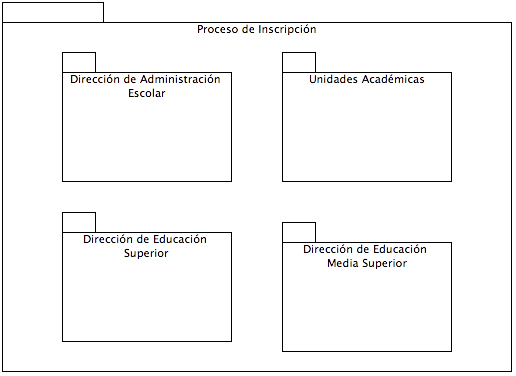
\includegraphics[width=0.7\textwidth]{dinamico/images/ArquitecturaLogica.png}}
		\caption{Diagrama de arquitectura lógica de inscripciones}
		\label{fig:arquitecturaIN}
	\end{center}
\end{figure}

%%		------------------------Diagrama de Dirección de Administración Escolar--------------------------
%		
%		La figura \ref{fig:PINDAE} muestra los submódulos para el módulo de la Dirección de Administración Escolar.\\
%		
%		\begin{figure}[htbp]
%			\begin{center}
%				\fbox{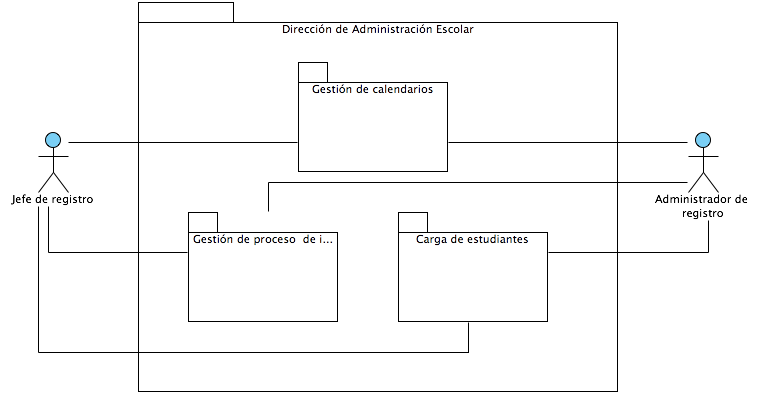
\includegraphics[width=0.9\textwidth]{dinamico/images/PIN_DAE.png}}
%				\caption{Módulo de la Dirección de Administración Escolar}
%				\label{fig:PINDAE}
%			\end{center}
%		\end{figure}
%	
%				La figura \ref{fig:PINDAEGestionDeCalendarios} muestra los casos de uso para el submódulo de Gestión de Calendarios, en el cual el \refElem{DAEAdministradorDeRegistro} podrá registrar la calendarización para las Unidades Académicas del Instituto.\\
%				
%				\begin{figure}[htbp]
%					\begin{center}
%						\fbox{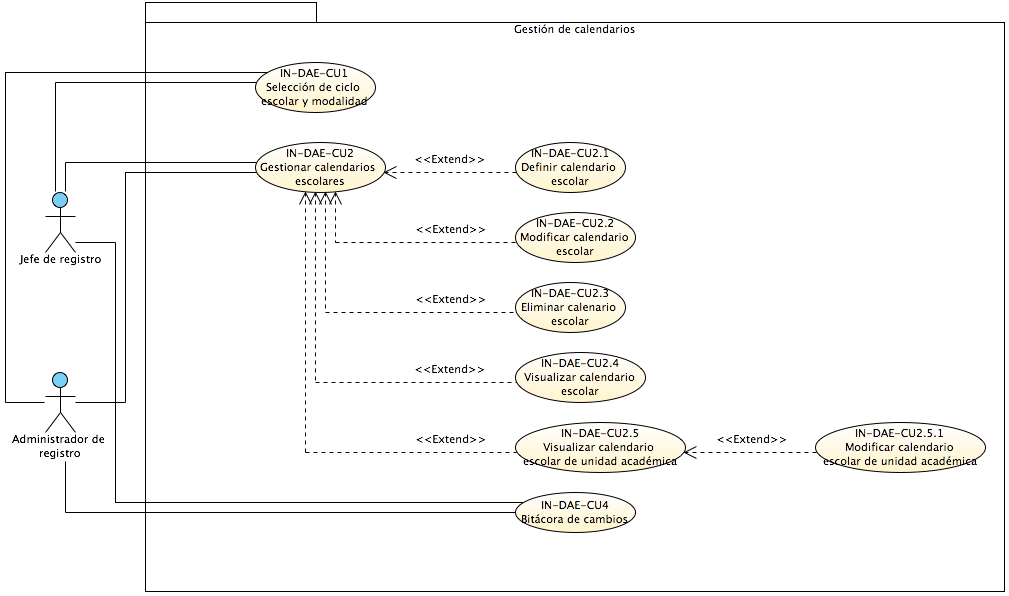
\includegraphics[width=0.9\textwidth]{dinamico/images/PIN_DAE_GestionDeCalendarios.png}}
%						\caption{Submódulo de Gestión de Calendarios}
%						\label{fig:PINDAEGestionDeCalendarios}
%					\end{center}
%				\end{figure}
%
%				La figura \ref{fig:PINDAEGestionDeProcesoDeInscripcion} muestra los casos de uso para el submódulo de Gestión de Proceso de Inscripción, en el cual el \refElem{DAEAdministradorDeRegistro} podrá administrar los procesos de inscripción registrados en el sistema, los cuales realizan la importación de estudiantes al Calmécac. \\
%
%				\begin{figure}[htbp]
%					\begin{center}
%						\fbox{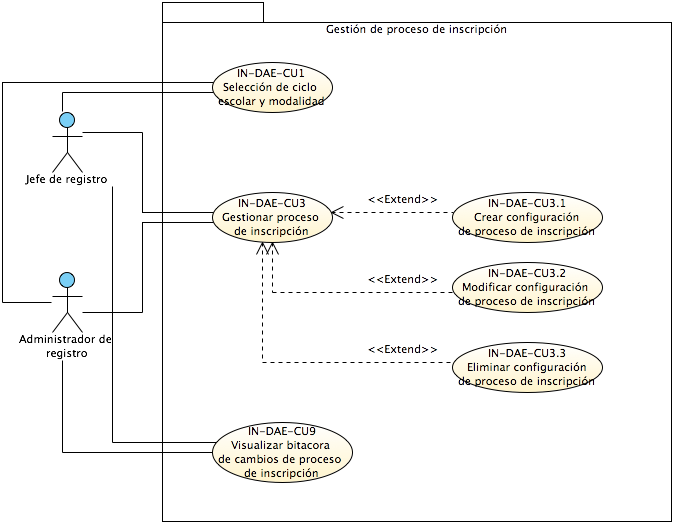
\includegraphics[width=0.9\textwidth]{dinamico/images/PIN_DAE_GestionDeProcesoDeInscripcion.png}}
%						\caption{Submódulo de Gestión de Proceso de Inscripción}
%						\label{fig:PINDAEGestionDeProcesoDeInscripcion}
%					\end{center}
%				\end{figure}
%			
%				La figura \ref{fig:PINDAECargaDeEstudiantes} muestra los casos de uso para el submódulo de Carga de Estudiantes, en el cual el \refElem{DAEAdministradorDeRegistro} podrá visualizar a los estudiantes de nuevo ingreso en el Instituto, estos pueden ser visualizados por Unidad Académica y Programa Académico.\\
%
%				\begin{figure}[htbp]
%					\begin{center}
%						\fbox{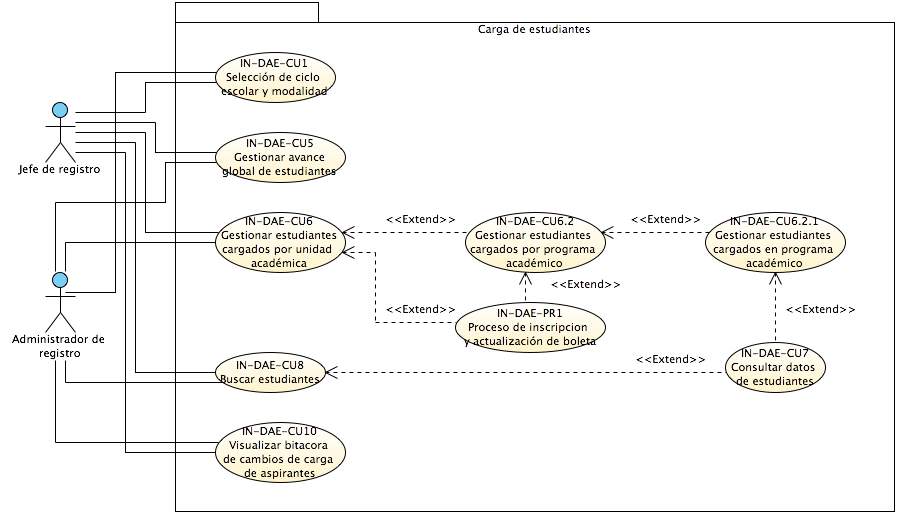
\includegraphics[width=0.9\textwidth]{dinamico/images/PIN_DAE_CargaDeEstudiantes.png}}
%						\caption{Submódulo de Carga de Estudiantes}
%						\label{fig:PINDAECargaDeEstudiantes}
%					\end{center}
%				\end{figure}
%			
%%		------------------------Diagrama de Dirección de Educación Superior--------------------------
%		
%		La figura \ref{fig:PINDES} muestra los submódulos para el módulo de la Dirección de Educación Superior.\\
%			
%		\begin{figure}[htbp]
%			\begin{center}
%				\fbox{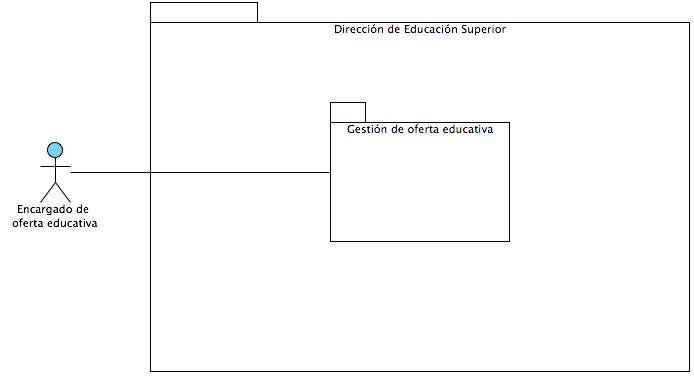
\includegraphics[width=0.9\textwidth]{dinamico/images/PIN_DES.png}}
%				\caption{Módulo de la Dirección de Educación Superior}
%				\label{fig:PINDES}
%			\end{center}
%		\end{figure}
%	
%				La figura \ref{fig:PINDESGestionDeOfertaEducativa} muestra los casos de uso para el submódulo de Gestión de Oferta Educativa, en el cual el \refElem{DESEncargadoDeOfertaEducativa} podrá registrar la oferta educativa para los Programas Académicos de las Unidades Académicas de nivel Superior.\\
%				
%				\begin{figure}[htbp]
%					\begin{center}
%						\fbox{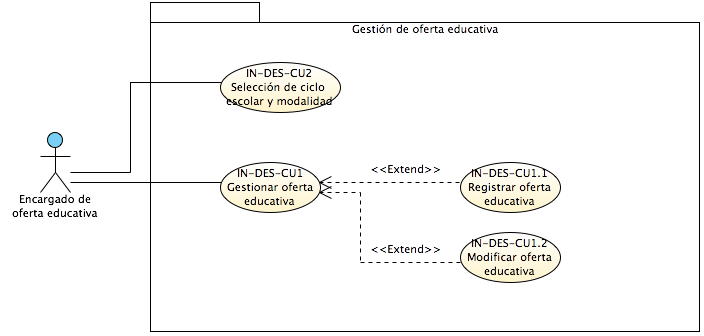
\includegraphics[width=0.9\textwidth]{dinamico/images/PIN_DES_GestionDeOfertaEducativa.png}}
%						\caption{Submódulo de Gestión de Oferta Educativa}
%						\label{fig:PINDESGestionDeOfertaEducativa}
%					\end{center}
%				\end{figure}
%				
%%		------------------------Diagrama de Dirección de Educación Media Superior--------------------------
%
%		La figura \ref{fig:PINDEMS} muestra los submódulos para el módulo de la Dirección de Educación Media Superior.\\
%		
%		\begin{figure}[htbp]
%			\begin{center}
%				\fbox{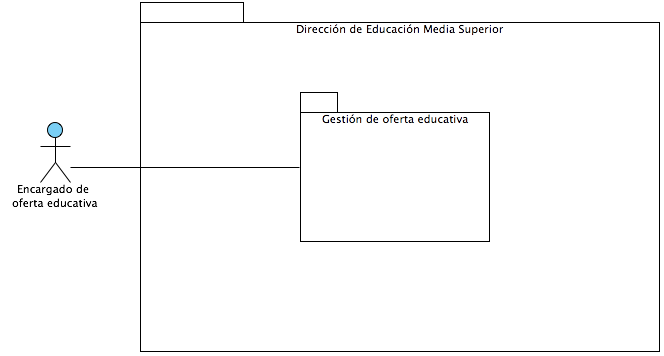
\includegraphics[width=0.9\textwidth]{dinamico/images/PIN_DEMS.png}}
%				\caption{Módulo de la Dirección de Educación Media Superior}
%				\label{fig:PINDEMS}
%			\end{center}
%		\end{figure}
%		
%				La figura \ref{fig:PINDEMSGestionDeOfertaEducativa} muestra los casos de uso para el submódulo de Gestión de Oferta Educativa, en el cual el \refElem{DESEncargadoDeOfertaEducativa} podrá registrar la oferta educativa para los Programas Académicos de las Unidades Académicas de nivel Superior.\\
%				
%				\begin{figure}[htbp]
%					\begin{center}
%						\fbox{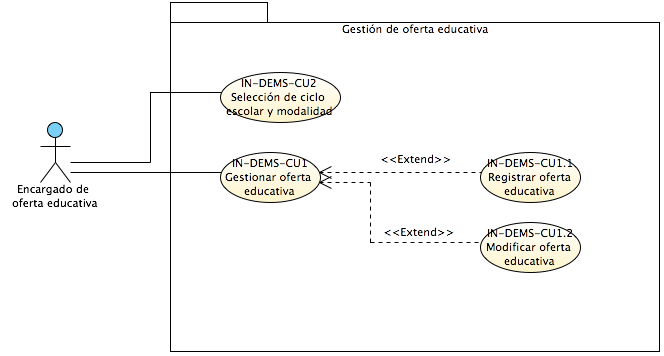
\includegraphics[width=0.9\textwidth]{dinamico/images/PIN_DEMS_GestionDeOfertaEducativa.png}}
%						\caption{Submódulo de Gestión de Oferta Educativa}
%						\label{fig:PINDEMSGestionDeOfertaEducativa}
%					\end{center}
%				\end{figure}
				
%		------------------------Diagrama de Unidad Académica --------------------------

		La figura \ref{fig:PINUA} muestra los submódulos para el módulo de Unidad Académica.\\
		
		\begin{figure}[htbp]
			\begin{center}
				\fbox{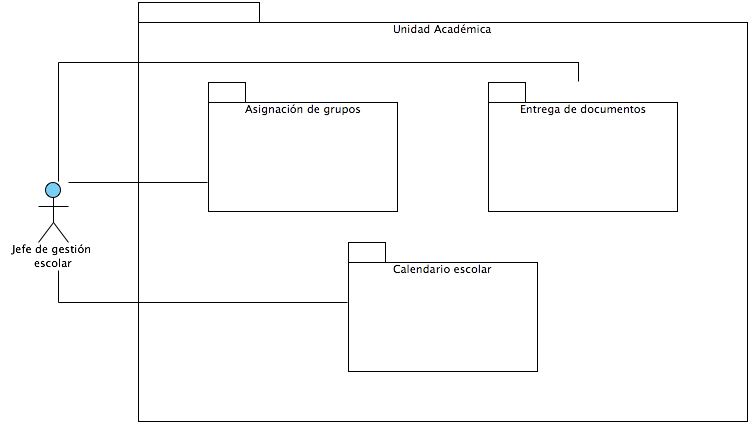
\includegraphics[width=0.9\textwidth]{dinamico/images/PIN_UA.png}}
				\caption{Módulo de Unidad Académica}
				\label{fig:PINUA}
			\end{center}
		\end{figure}
		
%				La figura \ref{fig:PINUAGestionDeCalendarios} muestra los casos de uso para el submódulo de Gestión de Calendarios, en el cual el \refElem{UAJefeDeGestionEscolar} podrá registrar la calendarización para su Unidad Académica.\\
%
%				\begin{figure}[htbp]
%					\begin{center}
%						\fbox{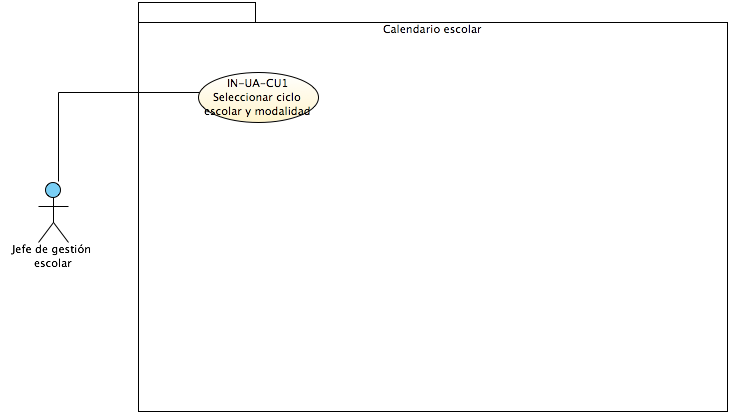
\includegraphics[width=0.9\textwidth]{dinamico/images/PIN_UA_CalendarioEscolar.png}}
%						\caption{Submódulo de Gestión de Calendarios}
%						\label{fig:PINUAGestionDeCalendarios}
%					\end{center}
%				\end{figure}
								
				La figura \ref{fig:PINUAAsignacionDeGrupos} muestra los casos de uso para el submódulo de Asignación de Grupos, en el cual el \refElem{UAJefeDeGestionEscolar} podrá asignarle grupos y Unidades de Aprendizaje a los estudiantes de nuevo ingreso de su Unidad Académica.\\

				\begin{figure}[htbp]
					\begin{center}
						\fbox{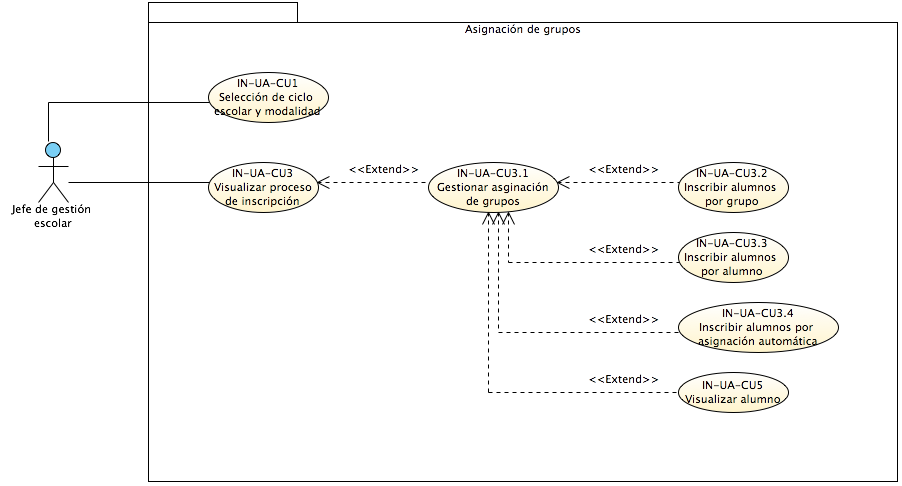
\includegraphics[width=0.9\textwidth]{dinamico/images/PIN_UA_AsignacionDeGrupos.png}}
						\caption{Submódulo de Asignación de Grupos}
						\label{fig:PINUAAsignacionDeGrupos}
					\end{center}
				\end{figure}

%				La figura \ref{fig:PINUAEntregaDeDocumentos} muestra los casos de uso para el submódulo de Entrega de Documentos, en el cual el \refElem{UAJefeDeGestionEscolar} podrá registrar la entrega de documentos de los estudiantes de nuevo ingreso.\\
%
%				\begin{figure}[htbp]
%					\begin{center}
%						\fbox{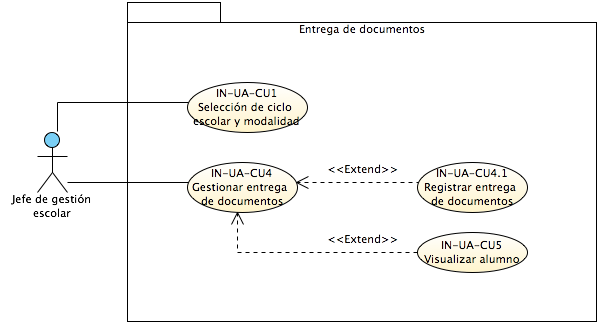
\includegraphics[width=0.9\textwidth]{dinamico/images/PIN_UA_EntregaDeDocumentos.png}}
%						\caption{Submódulo de Entrega de Documentos}
%						\label{fig:PINUAEntregaDeDocumentos}
%					\end{center}
%				\end{figure}